\section{User Interface Entwürfe}

Die User Interfaces wurden so gestaltet, dass sie die zuvor genannten User Stories, Use Cases und Anforderungen bestmöglich erfüllen. 
\paragraph{}Dabei werden die Mitarbeiter Use Cases in einer mobile first Anwendung verpackt, weil die Arbeitsplatzbuchungen schnell und leicht von der Hand gehen sollen.
Ebenfalls ist mobile first praktisch für die Nachtrichten-Funktion, da die Erreichbarkeit und die Möglichkeit schnell zu antworten, auf mobilen Geräten besser ist als auf Desktop Systemen. 
\paragraph{}Die Use Cases des Administrators und der Geschäftsführung werden wiederum auf Desktop-Systeme ausgelegt, da dort eine übersichtliche, effiziente und präzise Nutzung wichtiger ist, als die Flexibilität auf das System zuzugreifen zu können. 

\subsection{Mitarbeiter User Interface}

Nachfolgend werden die Funktionen und Seiten des mobile first User Interfaces visualisiert und erläutert. 

\subsubsection{Buchen}

\begin{wrapfigure}{r}{5.5cm}
    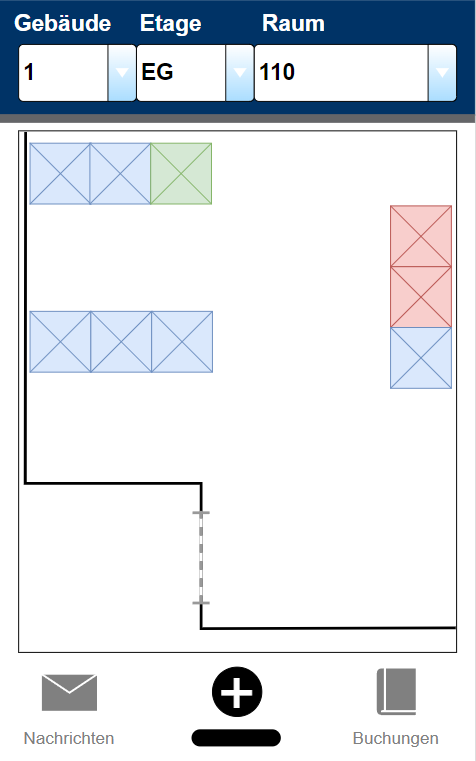
\includegraphics[width=5cm]{sketchBooking.png}
    \caption{User Interface: Buchen}
  \end{wrapfigure}

Sobald die Anwendung abgerufen wird, erhält man das Buchen-Fenster.
\paragraph{}Ersichtlich ist das aktuell geöffnete Fenster durch die Funktionsleiste am unteren Ende der Anwendung. 
Dort wird die ausgewählte Funktion, spricht das aktuelle Fenster, durch die dunkel schwarze Färbung und den Balken darunter hervorgehoben.
\paragraph{}Im oberen Teil der Anwendung kann man über Dropdown-Menus sich das Gebäude, die Etage und den Raum raussuchen, in dem mach buchen möchte.
Dabei wählt man von rechts startend aus, spricht zuerst das Gebäude, dann die Etage und zuletzt den Raum.

Dies ist wichtig, weil je nach Gebäude andere Etagen bestehen, welche dann wieder nur bestimmte Räume enthalten.
\paragraph{}Wenn im oberen Teil alle Angaben bis zum Raum hin gegeben wurden, sieht man in der Mitte der Anwendung den ausgewählten Raum.
Dieser wird durch ein Rechteck mit dünnen  schwarzen Linien in der Anwendung begrenzt.
In diesem Rahmen soll es möglich sein den Raum zu verschieben und zu vergrößern und zu verkleinern.
Der Raum an sich besteht zum einen aus Wänden, dicke schwarze Striche, und Türen, grau gestrichelte Einsätze in den Wänden. Türen und Wände werden 
lediglich zur Orientierung und besseren Vorstellung des Raumes genutzt. 
\paragraph{}In dem Raum befinden sich schließlich farbige Rechtecke, welche Arbeitsplätze darstellen, mit denen man interagieren kann. Die farbliche Kennzeichnung beschreibt, wie der Platz an dem heutigen Tag genutzt wird.
Blau zeigt an, dass der Platz frei verfügbar ist für heute, rot zeigt an, dass der Platz mindestens in einem Zeitfenster von heute eine Buchung eines anderen Arbeitskollegen vorliegen hat und grün zeigt an, dass man den Arbeitsplatz für heute selbst in mindestens einem Zeitfenster gebucht hat.
\paragraph{}Um weitere und genauere Informationen über die Belegung eines Arbeitsplatzes zu erhalten, klickt man diesen an.
